\section{2024年11月27日} % 日期作为章节显示在目录中

\subsection{今日进展} % 今日进展
1. 完成了棋盘初始化、显示、落子验证的实现。

2. 实现了胜负判断逻辑,通过检查横向、纵向、两种斜向的五子连珠状态,判断玩家是否获胜。

3. 实现了黑白棋的交替落子逻辑,并在有效落子后实时更新棋盘。

4. 优化了终端显示,解决了中文输出乱码问题。

\subsection{成果展示} % 成果展示

\subsubsection{程序界面截图}
\begin{figure}[h]
    \centering
    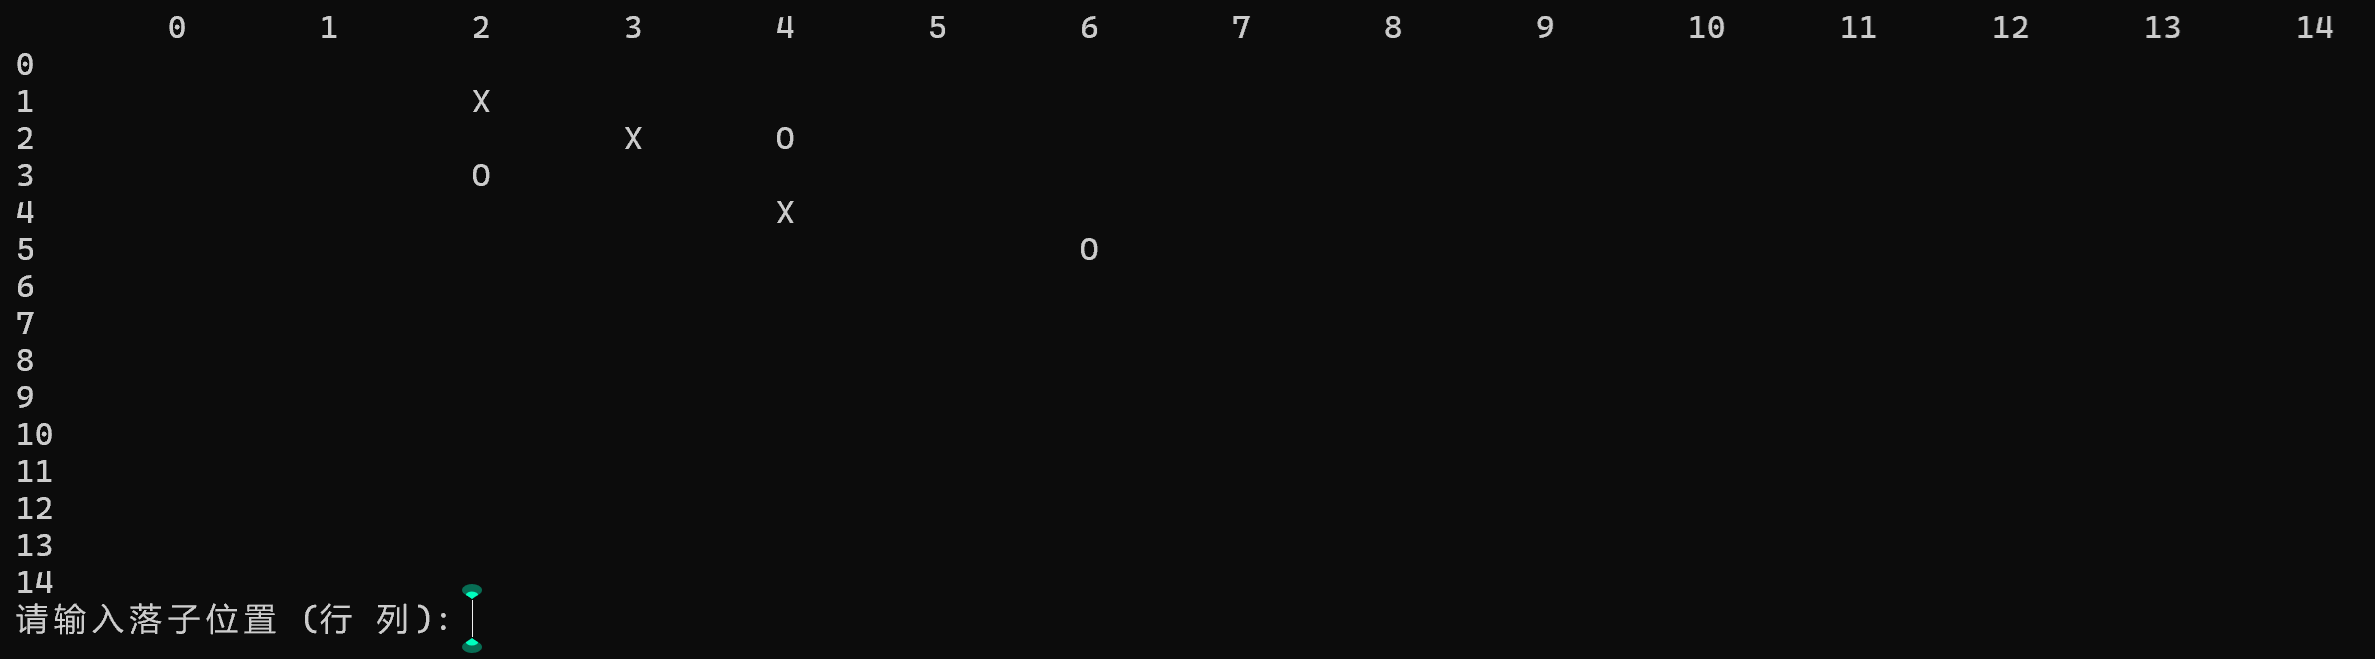
\includegraphics[width=0.7\textwidth]{logs/image/0001.png}
    \caption{程序运行截图}
    \label{fig:program_output}
\end{figure}

\subsubsection{运行结果}
程序成功运行,能够初始化指定大小的棋盘,支持黑白棋交替落子,并正确判断胜负。

\subsection{问题与解决方案} % 问题与解决方案

\subsubsection{遇到的问题}
1. 在终端中显示中文提示时出现乱码。

2. 无法确定落子是否形成五子连珠,导致游戏胜负判断逻辑缺失。

\subsubsection{解决方法}
1. 使用 `SetConsoleOutputCP(65001)` 将控制台编码设置为 UTF-8,解决了中文乱码问题。

2. 编写了 `checkwin` 函数,通过遍历四个方向检查当前玩家是否形成五子连珠。

\subsection{代码分析} % 代码分析

\subsubsection{棋盘初始化与显示}
\begin{lstlisting}[caption={棋盘初始化与显示代码}, label={code:board_init}]
vector<vector<char>> initializeBoard(int size) 
{
    return vector<vector<char>>(size, vector<char>(size, ' '));
}

void displayBoard(const vector<vector<char>>& board) 
{
    cout << "\t";
    for (int i = 0; i < board.size(); ++i) {
        cout << i << "\t";
    }
    cout << endl;

    for (int i = 0; i < board.size(); ++i) {
        cout << i << "\t";
        for (int j = 0; j < board[i].size(); ++j) {
            cout << board[i][j] << "\t";
        }
        cout << endl;
    }
}
\end{lstlisting}

\subsubsection{胜负判断核心代码}
\begin{lstlisting}[caption={五子连珠胜负判断代码}, label={code:win_check}]
bool checkwin(const vector<vector<char>>& board, int x, int y, int currentPlayer) {
    int directions[4][2] = {{1, 0}, {0, 1}, {1, 1}, {1, -1}};
    for (auto direction : directions) {
        int count = 1;

        for (int i = 1; i < 5; i++) {
            int nx = x + i * direction[0];
            int ny = y + i * direction[1];
            if (nx >= 0 && nx < board.size() && ny >= 0 && ny < board.size() && 
                board[nx][ny] == currentPlayerchar[currentPlayer]) {
                count++;
            } else {
                break;
            }
        }
        for (int i = 1; i < 5; i++) {
            int nx = x - i * direction[0];
            int ny = y - i * direction[1];
            if (nx >= 0 && nx < board.size() && ny >= 0 && ny < board.size() && 
                board[nx][ny] == currentPlayerchar[currentPlayer]) {
                count++;
            } else {
                break;
            }
        }
        if (count == 5) return true;
    }
    return false;
}
\end{lstlisting}

\subsection{明日计划} % 明日计划
1. 增加平局检测功能。

2. 实现黑棋禁手规则(如三三禁手、四四禁手)。

3. 为游戏添加菜单功能,支持重新开始或退出。


